\section{Solução desenvolvida}
\label{sec:iotGateway}

Além desse artigo, foi desenvolvida também uma solução de software para atingir os objetivos aqui propostos. O projeto está disponibilizado no Github \cite{IoTGatewayGithub} e essa seção se propõe a detalhar as decisões arquiteturais.

As decisões de tecnologia por trás da implementação do projeto foram feitas sempre com foco na portabilidade e execução em dispositivos com baixo recurso de memória e processamento. Portanto, selecionamos o seguinte conjunto de tecnologias:
\begin{itemize}
	\item Node.js v6.x \cite{NodeJS}
	\item TypeScript 2.3 com transpile para ES6 \cite{Typescript}
	\item TSLint 4.x com recomendações gerais padrão \cite{TSLint}
	\item Jest para teste unitário e cobertura \cite{Jest}
	\item Angular 1.6 para o front end da aplicação \cite{AngularJS}
	\item MongoDB \cite{MongoDB}
\end{itemize}

O node foi escolhido por conta de seu baixo consumo de memória e processamento, além do seu Non-Blocking IO, garantindo que possamos servir mais clientes com menos recursos, objetivo essencial para aplicações que podem ser executadas em um Raspberry Pi por exemplo. A intenção era ter uma estrutura tipada, de forma que a manutenção do código fosse facilitada e as regras de negócio pudessem estar ligadas a um contrato de objeto. Já o angular 1 foi escolhido, por ser uma tecnologia que funciona com javascript nativo, sem necessidade de nenhum pós-processador para servir a aplicação, permitindo o seu uso diretamente entre os arquivos estáticos do mesmo servidor Node.js que expõe a aplicação. Além disso, contou como um ponto para a escolha, a experiência prévia da equipe no desenvolvimento com este tipo de tecnologia. Decisões como a de não inserir nenhum processo de build, foram tomadas para que fosse possível servir o angular facilmente como um serviço estático do express.js

Modelo de Dados

O modelo de dados foi feito com a intenção de tornar a configuração de triggers para os eventos mais fácil e plugável. 

\begin{figure}
	\centering
	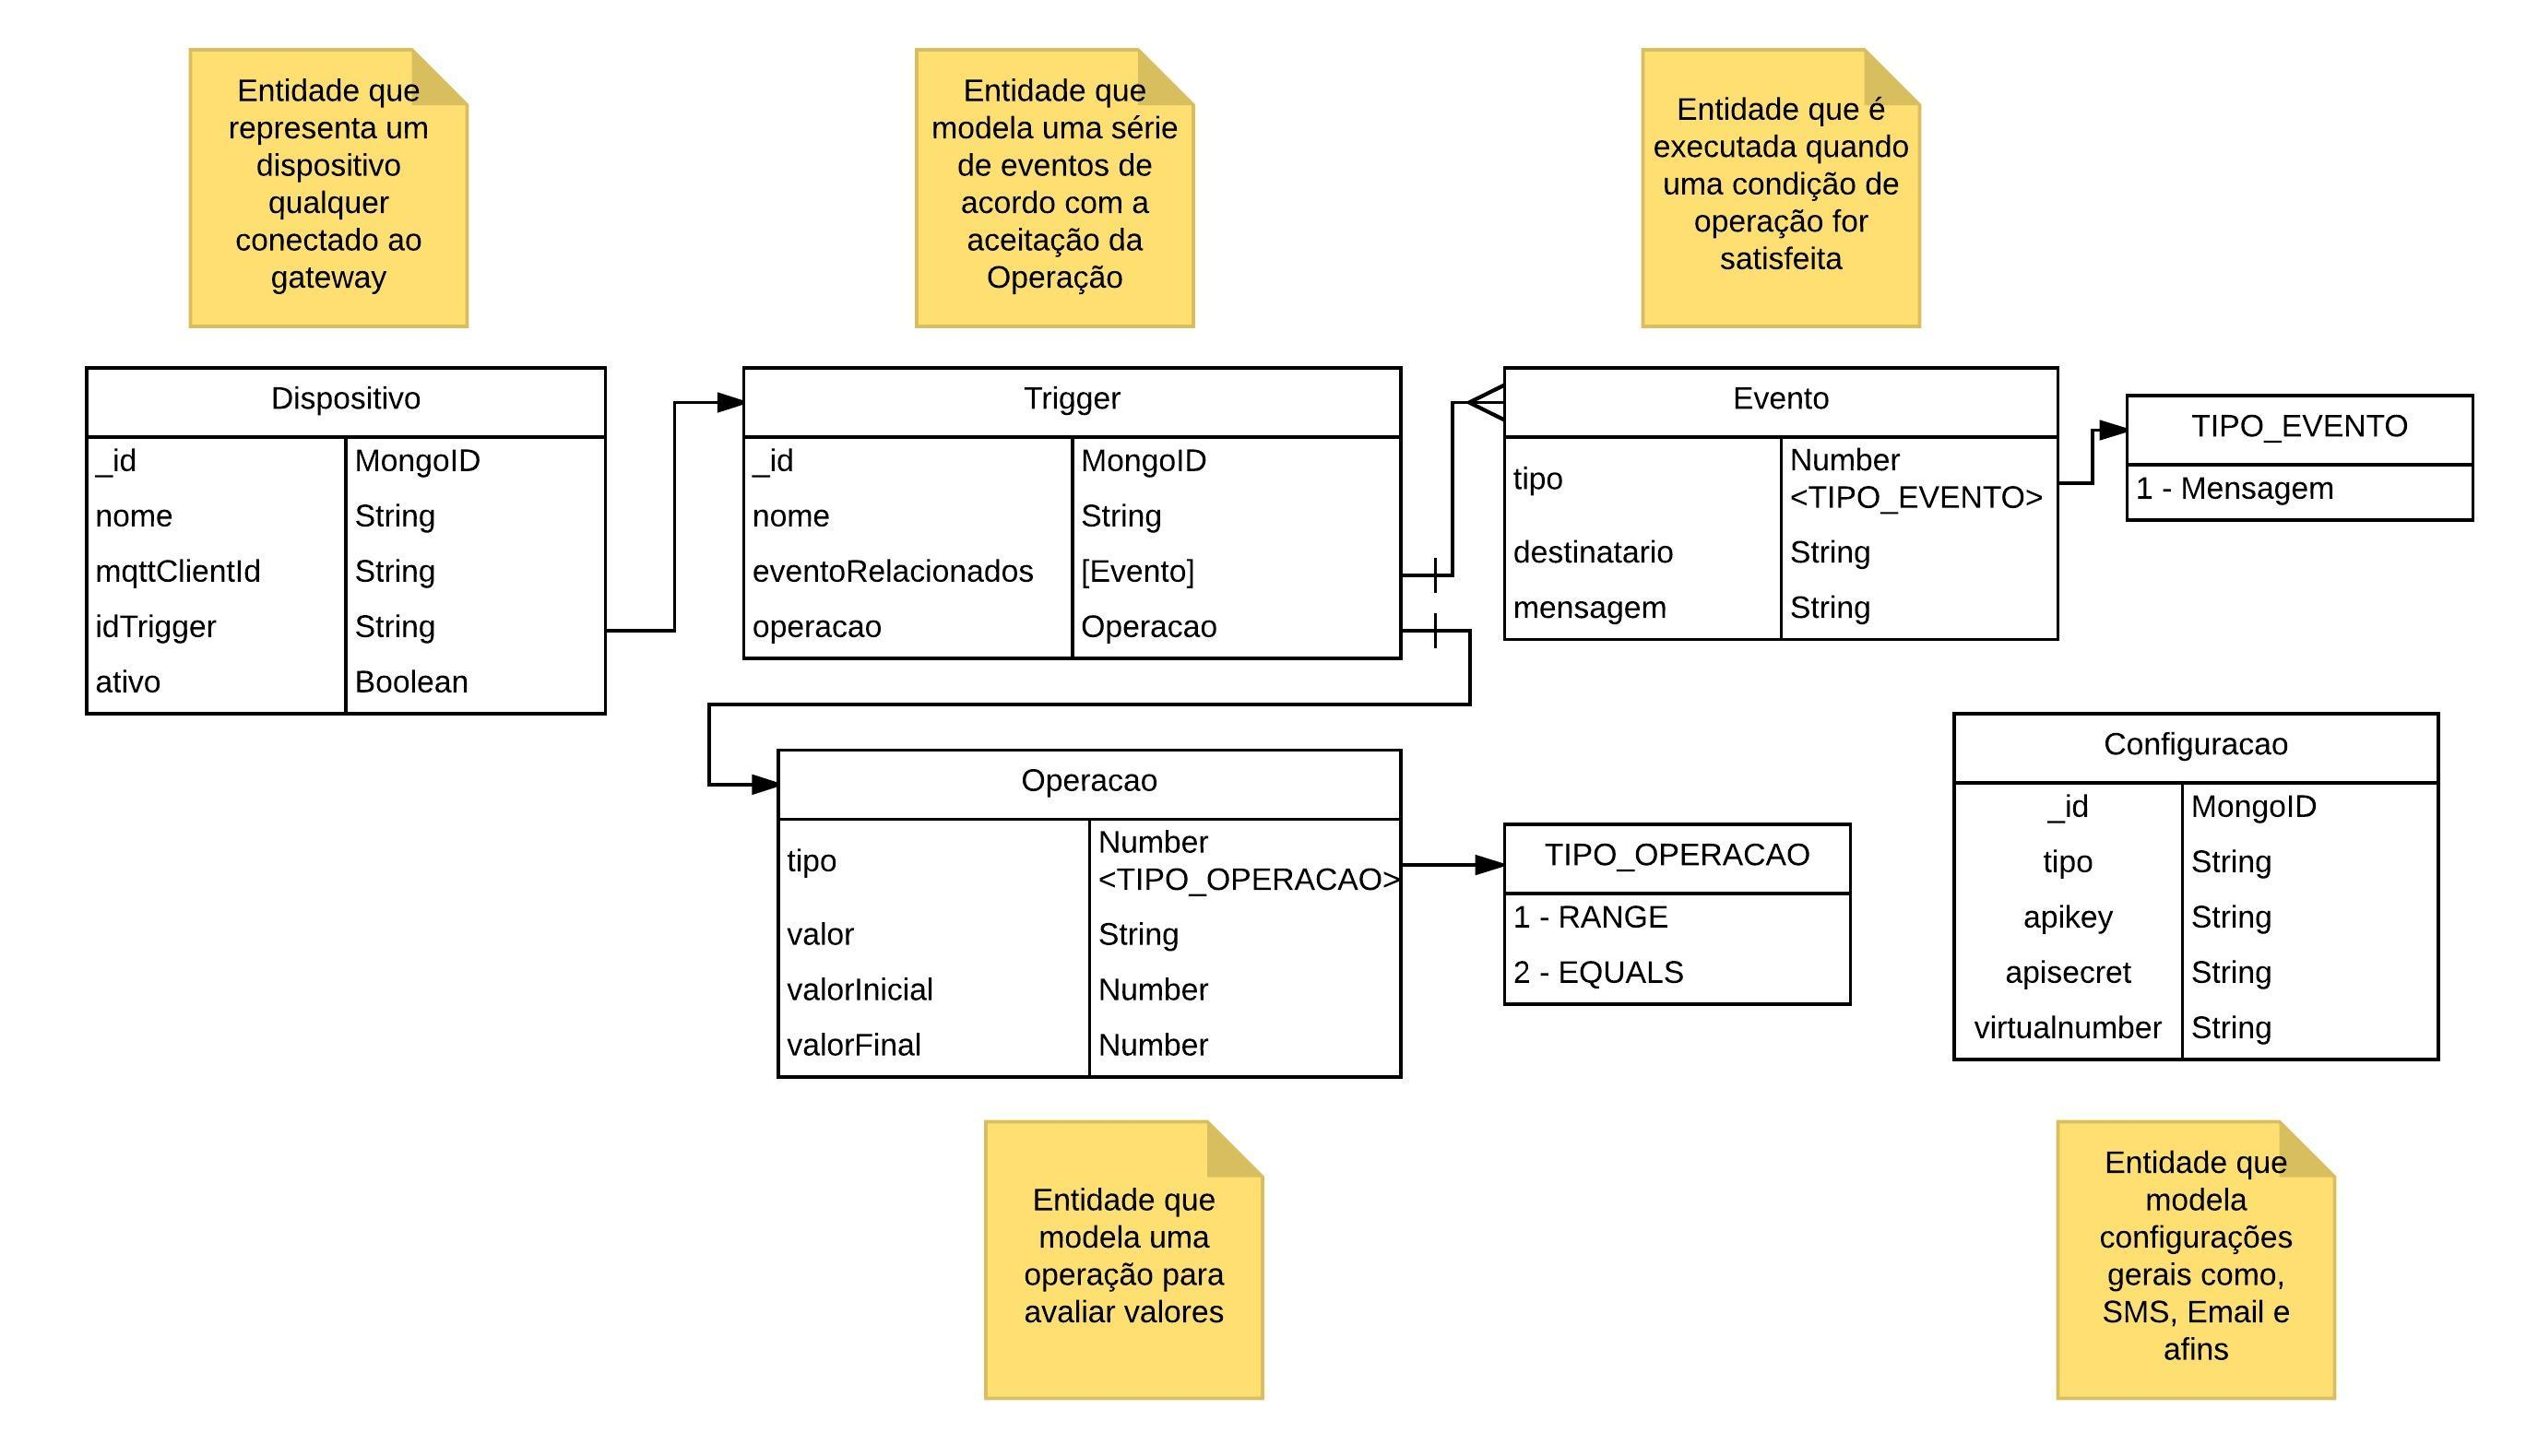
\includegraphics[width=1\textwidth]{./img/modelo-de-dados}
	\caption{Modelo de dados}
	\label{fig:modeloDeDados}
\end{figure}

Scripts disponíveis
\begin{verbatim}
npm start - Inicia o servidor do express.js;
npm clean - remove todos os caches e arquivos tranpilados;
npm build - Transpile de TypeScript para ES6;
npm run watch - Inicia um watch que efetua o transpile automatico de coisas alteradas;
npm lint - Executa um lint dos arquivos e dos testes;
npm test - Executa os testes;
npm test:watch - Inicia um watch que executa os testes sempre que algo for modificado;
\end{verbatim}

MongoDb, pode ser baixado através de imagem docker e executado da seguinte forma:
\begin{verbatim}
$ docker pull tutum/mongodb
$ docker run -d -p 27017:27017 -p 28017:28017 -e MONGODB_PASS="iot-gateway" tutum/mongodb
\end{verbatim}

Executando a aplicação
Execute o comando npm run watch em um console e deixe aberto
Execute o comando npm start em outro console
Abra o navegador na tela padrão conforme a porta configurada (ela será escrita no log, por padrão é 3000).
Carregando com dados básicos:

Os dados básicos para execução da app, são criados através de uma URL exposta no endpoint de api no endereço: \verb|http://localhost:3000/api/basicos|

Ao executar este endereço, será criado um cadastro wildcard, com ID do MQTT Client '*', de forma que qualquer dispositivo enviando os dados, terá seu cadastro de dispositivo atendido para este.

O evento padrão é o envio de SMS para o número padrão e será enviado sempre que a aplicação receber um valor \verb|true|	.